\documentclass[omni.tex]{subfiles}

\begin{document}

\begin{figure}
{\begin{center}
    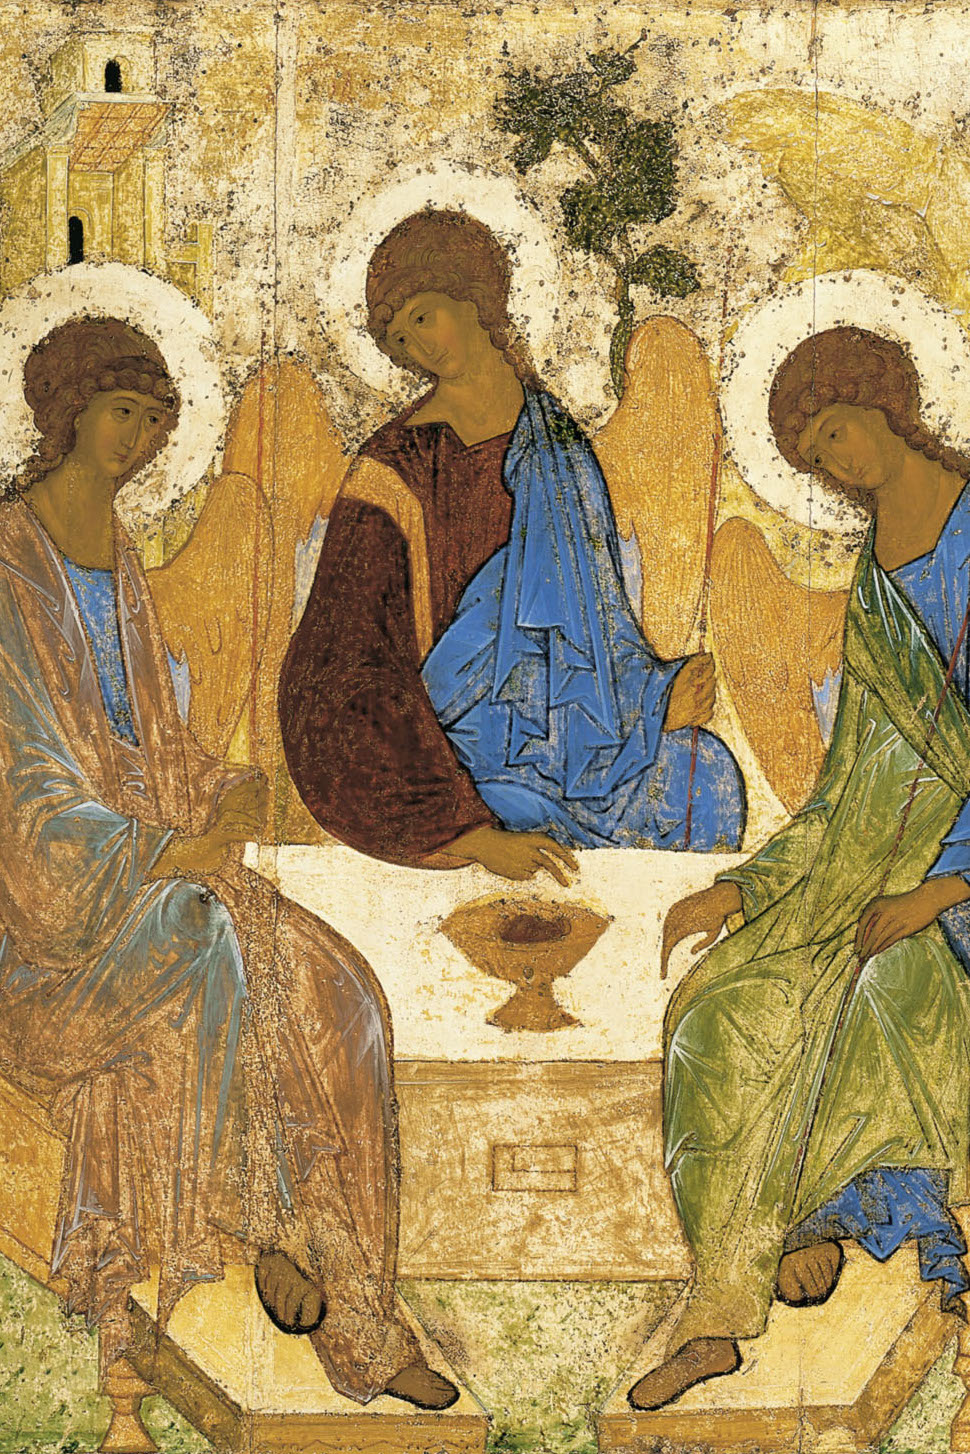
\includegraphics[width=2in]{trinity}
\end{center}}
\end{figure}

\poemtitle{Gl\'oria Patri}
\settowidth{\versewidth}{Et ne nos ind\'ucas in tentati\'onem}

\begin{verse}[\versewidth]
\lettrine[lhang=1.0,nindent=0em]{G}{l\'oria Patri}, \\>
et F\'ilio, \\>
et Spir\'itui Sancto.
\end{verse}

\begin{verse}[\versewidth]
Sicut erat in princ\'ipio \\
et nunc \\
et semper \\
et in s\ae cula s\ae culorum. \\
Amen. \\[7\baselineskip]
\end{verse}
\attrib{V}

\pagebreak
\end{document}
